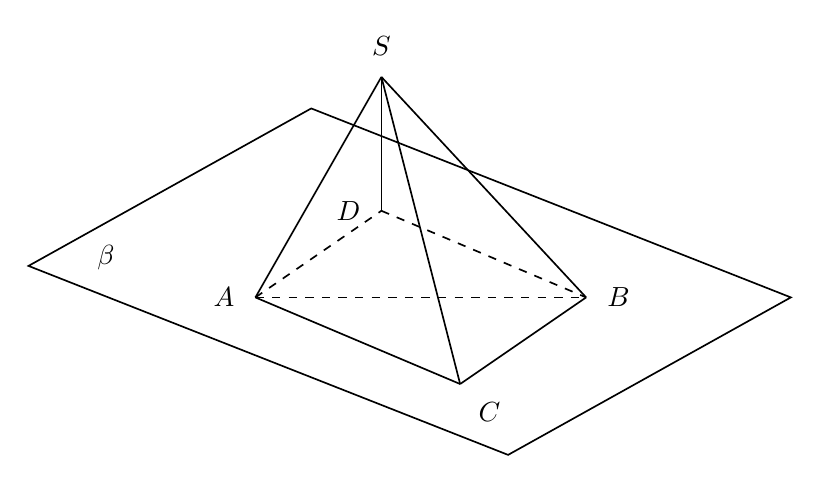
\begin{tikzpicture}[x=1cm,y=1cm,line width=0.6pt]
  % plane beta parallelogram
  \coordinate (P1) at (-4.1818181818,0.6000000000);
  \coordinate (P2) at (-0.5909090909,2.6000000000);
  \coordinate (P3) at (5.5000000000,0.2000000000);
  \coordinate (P4) at (1.9090909091,-1.8000000000);
  \draw[draw=black] (P1) -- (P2) -- (P3) -- (P4) -- cycle;
  \node[font=\normalsize] at (-3.2,0.7) {$\beta$};
  % pyramid points
  \coordinate (S) at (0.3000000000,3.0000000000);
  \coordinate (D) at (0.3000000000,1.3000000000);
  \coordinate (A) at (-1.3000000000,0.2000000000);
  \coordinate (B) at (2.9000000000,0.2000000000);
  \coordinate (C) at (1.3000000000,-0.9000000000);
  % foot and base dashed
  \draw[draw=black] (S) -- (D);
  \draw[draw=black,dashed] (A) -- (D);
  \draw[draw=black,dashed] (D) -- (B);
  \draw[draw=black,dashed] (A) -- (B);
  % base sides and apex
  \draw[draw=black] (A) -- (C);
  \draw[draw=black] (B) -- (C);
  \draw[draw=black] (S) -- (A);
  \draw[draw=black] (S) -- (B);
  \draw[draw=black] (S) -- (C);
  % labels with clearance
  \node[font=\normalsize,above=4pt] at (S) {$S$};
  \node[font=\normalsize,left=4pt] at (D) {$D$};
  \node[font=\normalsize,left=4pt] at (A) {$A$};
  \node[font=\normalsize,right=4pt] at (B) {$B$};
  \node[font=\normalsize,below right=3pt] at (C) {$C$};
\end{tikzpicture}
